% Sección 3 del informe técnico final: es la sección de metodología del Entregable 2
% (documentos/metodologia/metodologia.tex) copiada tal cual. Solo cambian, para encajarla en el informe,
% este encabezado, la última frase del primer párrafo y la línea \input de la subsección de decisión
% (secciones/03b_decision.tex), que va antes de «Disponibilidad de código y datos».
\section{Metodología}
\label{sec:metodologia}

Esta sección describe el problema, los datos, el modelo propuesto, su entrenamiento, los modelos de
referencia, el protocolo de comparación y el diseño del estudio de ablación y, al final, cómo el pronóstico
se convierte en decisiones de despacho (sección~\ref{sec:decision}); las cifras de desempeño se
reservan para la sección de resultados.

\subsection{Formulación del problema y notación}
\label{sec:formulacion}

Sobusa fija hoy las salidas de cada ruta y hora con el promedio de las ocho semanas anteriores para la misma
ruta, hora y día de la semana; la unidad de decisión, y por tanto de pronóstico, es la terna
\emph{ruta $\times$ día $\times$ hora de salida}.

Sea $r$ la ruta (SILENCIO, CRA~54 o CL~72), $d$ el día calendario y $h \in \{4, 5, \dots, 20\}$ la hora de
salida programada. La variable objetivo $y_{r,d,h} \in \mathbb{N}_0$ es el número de pasajeros transportados
por los viajes válidos que salen en esa franja. Como el horario semanal se programa con una semana de
antelación, el pronóstico operativo se emite con antelación $H \geq 7$ días: en el momento de emitirlo solo
se conoce la información hasta el día $d - H$; la antelación $H = 1$ se evalúa como referencia. El vector de
entrada $\bm{x}_{r,d,h} \in \X \subset \R^{p}$ se construye únicamente con esa información (rezagos de al
menos $H$ días), con el calendario, que se conoce de antemano, y con la climatología histórica. Se busca una
función $F: \X \to \R$ tal que $\yhat_{r,d,h} = \exp F(\bm{x}_{r,d,h})$ aproxime la esperanza condicional
$\E[\,y_{r,d,h} \mid \bm{x}_{r,d,h}\,]$. Es un problema de regresión supervisada de conteos sobredispersos
(razón varianza/media de 489 en el entrenamiento), así que la función de pérdida es la log-verosimilitud
negativa de Poisson con enlace logarítmico, ponderada por pesos de muestra $w_i$ que se definen en la
sección~\ref{sec:modelo}:
\begin{equation}
  \mathcal{L}(F) = \sum_{i=1}^{n} w_i \left[ \exp\!\big(F(\bm{x}_i)\big) - y_i\, F(\bm{x}_i) \right],
  \qquad \yhat_i = \exp\!\big(F(\bm{x}_i)\big),
  \label{eq:poisson}
\end{equation}
donde $n$ es el número de franjas de entrenamiento; la devianza de Poisson equivalente, sin pesos,
$D = 2\sum_i [\,y_i \ln(y_i/\yhat_i) - (y_i - \yhat_i)\,]$, se usa también como métrica. Aguas abajo,
el pronóstico se traduce a carga crítica prevista, $\hat{L}_{r,d,h} = \gamma_{r,h}\, \yhat_{r,d,h}$, con
$\gamma_{r,h}$ el cociente entre la carga del tramo más cargado del recorrido y los pasajeros de la franja,
medido por ruta y hora en 2023--2024 (medias por ruta de 0,40 en SILENCIO y CL~72 y 0,44 en CRA~54), y los
buses necesarios en la hora son
\begin{equation}
  N_{r,d,h} = \left\lceil \frac{\hat{L}_{r,d,h}}{Q\,\alpha} \right\rceil,
  \qquad Q = 50 \text{ pasajeros por bus},\ \alpha = 0{,}85,
  \label{eq:buses}
\end{equation}
donde $Q$ es la capacidad mediana de la flota y $\alpha$ el factor de carga objetivo (métrica de decisión
de la sección~\ref{sec:protocolo}); la tabla~\ref{tab:notacion} resume la notación.

\begin{table}[t]
  \centering\small
  \caption{Notación principal de la sección.}
  \label{tab:notacion}
  \begin{tabular}{@{}>{\raggedright\arraybackslash}p{0.2\linewidth} >{\raggedright\arraybackslash}p{0.74\linewidth}@{}}
    \toprule
    Símbolo & Significado \\
    \midrule
    $r, d, h$ & ruta, día calendario y hora de salida programada ($h \in \{4,\dots,20\}$) \\
    $j = (r, h)$ & una de las $51 = 3 \times 17$ series diarias ruta $\times$ hora \\
    $y_{r,d,h}$ & pasajeros de los viajes válidos que salen en la franja (objetivo, con ceros) \\
    $\tilde{y}_{r,d,h}$ & serie corregida por viajes sin registro, de la que se calculan los rezagos de pasajeros (ecuación~\eqref{eq:correccion}) \\
    $\phi_{r,d,h}$ & fracción de viajes válidos de la franja sin registro de pasajeros \\
    $H$ & antelación del pronóstico en días ($H = 7$ en la evaluación principal; también $1$, $14$, $21$ y $28$) \\
    $c = d - H$ & corte de información: último día que puede usar el pronóstico de $d$ \\
    $\bm{x}_i \in \R^{p}$ & vector de variables de la franja $i$; $p = 77$ para $H = 7$ y $92$ para $H = 1$ \\
    $n$ & número de franjas de entrenamiento \\
    $F(\bm{x})$ & suma de $T$ árboles de regresión (ecuación~\eqref{eq:gbm}); $\yhat = \exp F(\bm{x})$ \\
    $w_i$ & peso de muestra en el entrenamiento ($1$; $0{,}25$; $0{,}1$) \\
    $m$ & pliegue mensual de prueba ($m = 1,\dots,12$, meses de 2025) \\
    $\rho$ & coeficiente de correlación de Pearson \\
    $\wape, \mae, \rmse$ & métricas de la sección~\ref{sec:protocolo} \\
    $\hat{L}, \gamma_{r,h}$ & carga crítica prevista y cociente carga crítica / pasajeros de la ruta y hora \\
    $N, Q, \alpha$ & buses necesarios por hora, capacidad de un bus (50) y factor de carga objetivo (0,85) \\
    \bottomrule
  \end{tabular}
\end{table}

\subsection{Datos, análisis exploratorio y preprocesamiento}
\label{sec:datos}

\paragraph{Fuente y tamaño.}
Los datos son la base operativa de Sobusa para el \emph{Data Challenge}: una base PostgreSQL con PostGIS en
Amazon RDS (44~GB, solo lectura), con 175.855.828 eventos GPS agregados en el servidor. El periodo es del 1
de enero de 2023 al 31 de diciembre de 2025 (1.096 días, sin huecos) para las tres rutas: 564.832 viajes
programados con salida entre las 4 y las 20~h, de los que 520.638 son
válidos. Se cedieron bajo confidencialidad, no se redistribuyen y ninguna columna con datos personales entra
en la tabla de modelado. El clima proviene de Open-Meteo (licencia CC~BY~4.0) y los calendarios escolar y
universitario, de resoluciones oficiales y de las universidades de la ciudad.

\paragraph{Variable objetivo.}
$y_{r,d,h}$ es la suma de pasajeros de los viajes válidos con conteo (menor o igual que 300) que salen en la
franja; los ceros se conservan. La tabla de modelado tiene $55.896 = 3 \times 1.096 \times 17$ filas y el
conjunto de prueba de 2025, 18.615 franjas. En el entrenamiento (2023--2024, 37.179 franjas) el objetivo
tiene media 787, mediana 604, percentiles 10 y 90 de 201 y 1.742, máximo 3.680 y un 2,2~\% de ceros; su
asimetría (1,40) pasaría a $-2{,}96$ con $\log(1+y)$, así que no se transforma y se modela como conteo. Los
totales anuales bajan de 15,31 a 13,99 y a 12,87 millones de pasajeros, cerca de $-8$~\% al año con casi la
misma flota (figura~\ref{fig:datos}).

\begin{figure}[t]
  \centering
  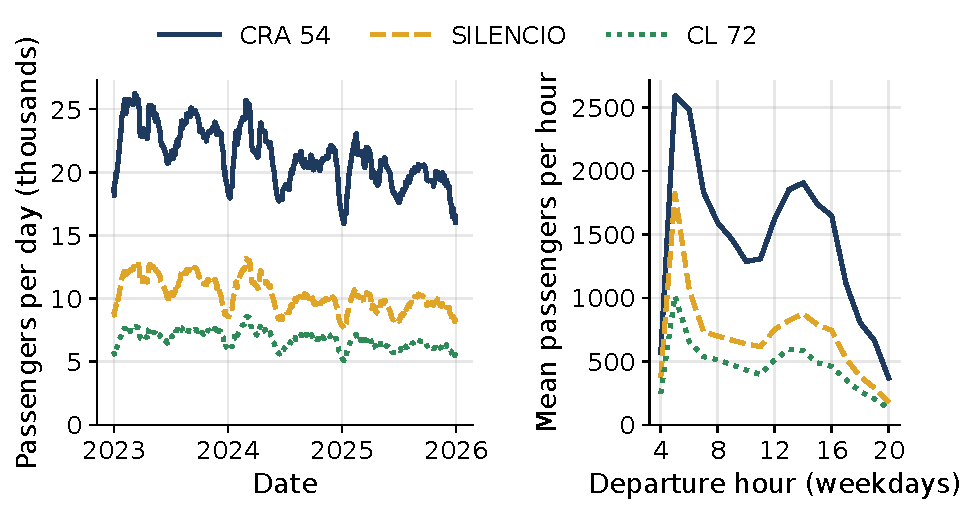
\includegraphics[width=\linewidth]{fig_demand_profile.pdf}
  \caption{Demanda de las tres rutas en la tabla de modelado. Izquierda: pasajeros por día (media móvil
  centrada de 28 días), 2023--2025. Derecha: pasajeros medios por hora de salida en días laborales.}
  \label{fig:datos}
\end{figure}

\paragraph{Hallazgos del análisis exploratorio que guían el modelado.}
Las correlaciones, los tamaños de efecto y las autocorrelaciones se calcularon solo con 2023--2024; 2025 se
reservó como prueba antes de mirar el objetivo. La estacionalidad dominante es semanal (autocorrelación de
0,62--0,65 a 7 días frente a 0,31--0,37 a 1 día). El sábado mueve el 81~\% de un día laboral y el domingo o
festivo el 39--42~\%; los festivos entre semana caen un 62--65~\%, el Carnaval hasta un 79~\% y las
vacaciones escolares y universitarias entre un 8 y un 21~\%. Las tres rutas están muy correlacionadas
($\rho \geq 0{,}96$), de ahí un único modelo con la ruta como categórica. La lluvia explica menos
del 2~\% de la varianza y no se pronostica a siete días, así que entra solo como climatología. La regla
manual de las ocho semanas es la variable más correlacionada con el objetivo ($\rho = 0{,}90$): variable y
línea base a la vez.

\paragraph{Limpieza.}
La tabla~\ref{tab:limpieza} resume las reglas, numeradas como en el Entregable~1.

\begin{table}[t]
  \centering\small
  \caption{Reglas de limpieza y de construcción de la tabla de modelado.}
  \label{tab:limpieza}
  \begin{tabular}{@{}l >{\raggedright\arraybackslash}p{0.86\linewidth}@{}}
    \toprule
    Regla & Contenido \\
    \midrule
    R1 & viaje válido: finalizado y no cancelado (520.638 de 564.832) \\
    R2--R3 & para promedios por viaje: duración de 30 a 360 minutos y de 1 a 300 pasajeros (490.318 viajes); el filtro de distancia de 45--80~km previsto en R3 no se adopta \\
    R4 & objetivo: suma por franja de los viajes válidos con conteo $\leq 300$; los ceros se conservan \\
    R5 & dos días fuera del entrenamiento y de las líneas base: paro del 6-9-2024 ($-82{,}8$~\%) y falla de registro del 22-9-2024 ($-39{,}9$~\%) \\
    R7 & calendario con 53 festivos (paquete \texttt{holidays}) y 12 días de Carnaval \\
    R9 & ocupación GPS solo con contadores consistentes \\
    R11 & ninguna imputación del objetivo ni de las variables; los vacíos quedan como faltantes \\
    R12 & partición temporal; rezagos no menores que la antelación $H$ \\
    R13 & sin identificadores de conductor, vehículo ni despachador \\
    R14 & los atípicos de demanda no se eliminan \\
    \bottomrule
  \end{tabular}
\end{table}

\paragraph{Ingeniería de variables.}
La tabla de modelado reúne 129 columnas en 17 familias; el modelo usa 77 variables para $H = 7$ (92 para
$H = 1$), agrupadas en la tabla~\ref{tab:variables}. Los rezagos se calculan sobre la rejilla diaria de cada
serie ruta~$\times$~hora y solo se admiten los de $H$ días o más. La oferta entra solo rezagada (la del
día pronosticado es la decisión misma). Las categóricas
(ruta, día de la semana, tipo de día) se pasan como tales al modelo de árboles y ninguna variable se escala.
La corrección de rezagos y los pesos de muestra se definen en la sección~\ref{sec:modelo}.

\begin{table}[t]
  \centering\small
  \caption{Variables del modelo ($H = 7$) por familia. Todas se conocen con $H$ días de antelación.}
  \label{tab:variables}
  \begin{tabular}{@{}>{\raggedright\arraybackslash}p{0.27\linewidth} r >{\raggedright\arraybackslash}p{0.6\linewidth}@{}}
    \toprule
    Familia & Núm. & Variables \\
    \midrule
    Calendario base & 12 & ruta, hora, día de la semana, tipo de día, mes, día del mes, día del año, semana del año, tendencia, festivo, vacaciones, quincena \\
    Calendario especial & 6 & Carnaval, Carnaval central, Semana Santa, Jueves y Viernes Santo, 1 de enero, Navidad \\
    Eventos & 4 & partido y otro evento masivo, en el día y en la franja \\
    Rezagos ($4 \times 10$) & 40 & para pasajeros totales, pasajeros por viaje, carga máxima y viajes válidos: rezagos de 7, 14, 21 y 28 días, media de las cuatro mismas semanas, medias móviles de 7 y 28 días que terminan en $d-7$, regla de 8 semanas (B1), su desviación y rezago de 364 días \\
    Totales diarios de la ruta & 5 & pasajeros y viajes de la ruta en $d-7$ y $d-14$ y media móvil de 7 días \\
    Calendario escolar y de pago & 6 & vacaciones escolares y universitarias, fracción de la ventana de rezagos en vacaciones o en días especiales, días desde el último pago \\
    Climatología & 4 & temporada, lluvia media y probabilidad de lluvia por mes y hora, lluvia esperada en el viaje \\
    \bottomrule
  \end{tabular}
\end{table}

\paragraph{Particiones y control de fugas.}
La evaluación usa doce pliegues mensuales de 2025 con origen rodante: el mes $m$ es la prueba y el
entrenamiento usa todos los días estrictamente anteriores, de 36.821 filas en enero (las franjas de
2023--2024 con media de cuatro semanas) a 53.855 en diciembre (figura~\ref{fig:pliegues}). Las
configuraciones se fijaron de antemano o con ventanas de 2024 (secciones~\ref{sec:entrenamiento}
y~\ref{sec:referencias}); la selección entre variantes y candidatos usa los doce pliegues con la regla de la
sección~\ref{sec:protocolo}, y los finalistas se repiten en 2024. Ningún
estadístico de preprocesamiento usa datos de prueba: no hay escalado ni imputación, la climatología es de
2013--2022, los calendarios son públicos y los perfiles de las líneas base se recalculan en cada pliegue. Una
prueba de perturbación comprueba que, al alterar los datos desde una fecha $d_0$, ninguna variable de un día
anterior a $d_0 + H$ cambia, y cada predicción guarda su corte $c$, que el evaluador verifica
($d - c \geq H$). Los parámetros se ajustan con todos los días anteriores al mes de prueba (para los
primeros $H - 1$ días del mes, hasta $H - 1$ días después de su corte de variables), igual para todos los
modelos comparados.

\begin{figure}[tbp]
  \centering
  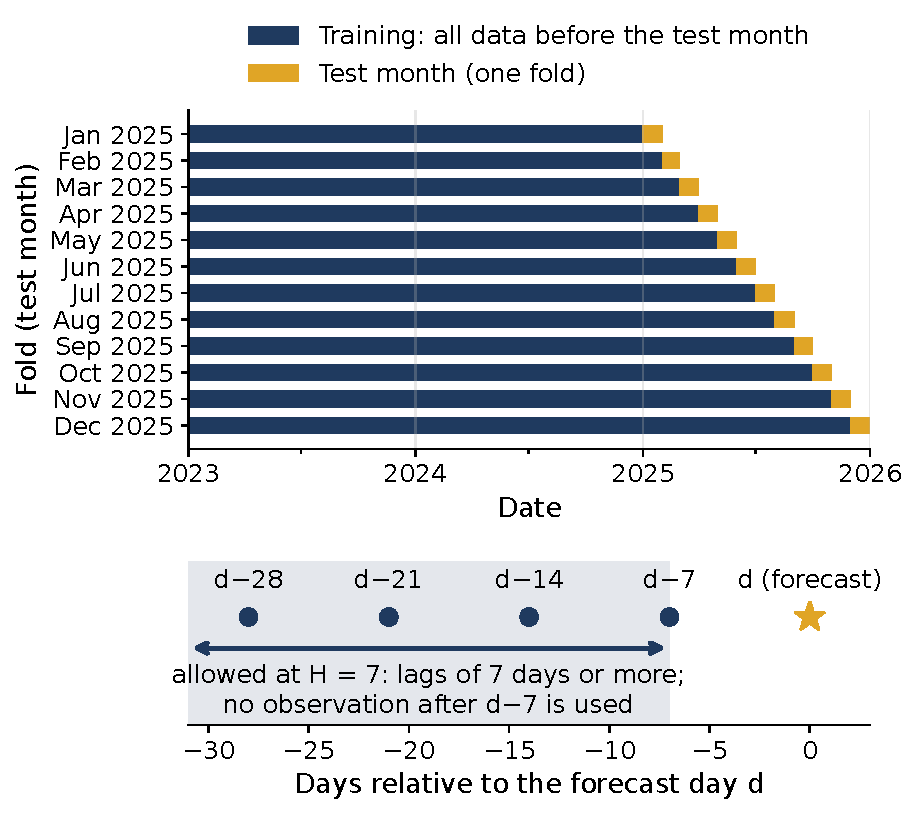
\includegraphics[width=\linewidth]{fig_rolling_folds.pdf}
  \caption{Protocolo de validación. Arriba: los doce pliegues mensuales de 2025 con origen rodante; cada mes
  se pronostica con un modelo entrenado solo con los días anteriores. Abajo: información admitida para
  pronosticar el día $d$ con antelación $H = 7$: rezagos de 7 días o más (puntos) y ninguna observación
  posterior a $d - 7$.}
  \label{fig:pliegues}
\end{figure}

\subsection{Modelo propuesto}
\label{sec:modelo}

\paragraph{Idea central.}
El modelo propuesto es una regresión de Poisson por \emph{gradient boosting} de árboles (LightGBM) sobre las
77 variables de ingeniería, con tres decisiones que lo distinguen de un \emph{boosting} estándar sobre la
tabla de modelado: (i)~los rezagos de pasajeros se calculan sobre una serie corregida por las fallas del
equipo de registro, (ii)~las filas con datos corruptos o atípicos reciben un peso bajo en lugar de imputarse
o excluirse, y (iii)~el calendario escolar y universitario entra como variables del día y como fracción de
la ventana de rezagos, para que el modelo sepa en qué régimen se midieron las referencias que usa. La
figura~\ref{fig:modelo} muestra la cadena completa.

\begin{figure}[tbp]
  \centering
  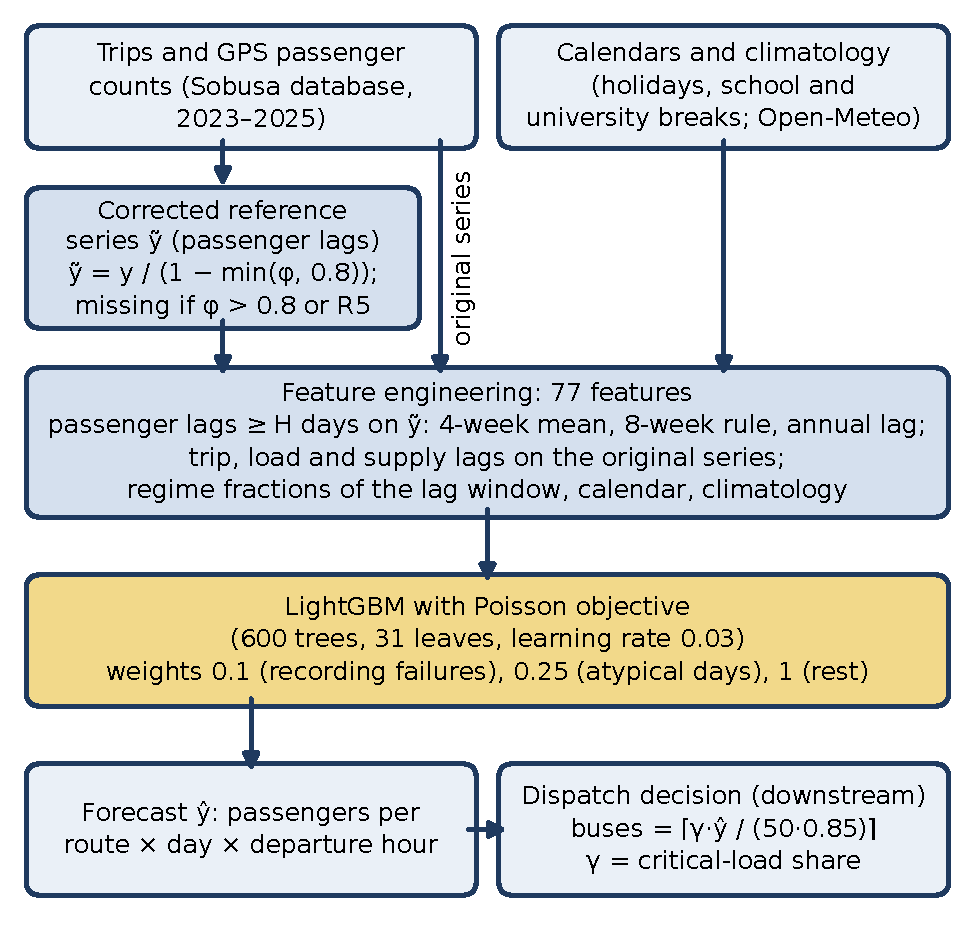
\includegraphics[width=\linewidth]{fig_model_pipeline.pdf}
  \caption{Arquitectura del modelo propuesto: de las fuentes de datos a las 77 variables, con los rezagos
  de pasajeros calculados sobre la serie corregida, los pesos de muestra y el LightGBM con objetivo de
  Poisson. El pronóstico alimenta la decisión de despacho de la ecuación~\eqref{eq:buses}.}
  \label{fig:modelo}
\end{figure}

\paragraph{Modelo de árboles.}
La función $F$ de la ecuación~\eqref{eq:poisson} es una suma de $T$ árboles de regresión ajustados por etapas
\citep{friedman2001gbm}:
\begin{equation}
  F_T(\bm{x}) = F_0 + \nu \sum_{t=1}^{T} f_t(\bm{x}), \qquad
  f_t = \arg\min_{f \in \mathcal{T}} \sum_{i=1}^{n} \tfrac{1}{2}\, w_i\, \eta_i^{(t)} \big( f(\bm{x}_i) - g_i^{(t)}/\eta_i^{(t)} \big)^2
  + \tfrac{\lambda}{2} \sum_{\ell} \theta_{\ell}^{2},
  \label{eq:gbm}
\end{equation}
donde $\nu$ es la tasa de aprendizaje, $\mathcal{T}$ la clase de árboles con a lo sumo 31 hojas, $\theta_\ell$
el valor de la hoja $\ell$ y $\lambda$ su penalización $\ell_2$, $F_0$ el logaritmo de la media ponderada del
objetivo, $g_i^{(t)} = y_i - \exp(F_{t-1}(\bm{x}_i))$ es el gradiente negativo (pseudorresiduo) de
\eqref{eq:poisson} y $\eta_i^{(t)} = \exp(F_{t-1}(\bm{x}_i) + \delta)$ su curvatura, con $\delta = 0{,}7$
para estabilizar el paso de Newton. LightGBM resuelve \eqref{eq:gbm} con histogramas de 255 cajas por
variable y crecimiento por hojas \citep{ke2017lightgbm}. La familia se eligió por los efectos no lineales y
de interacción (hora $\times$ tipo de día $\times$ vacaciones) que muestra el análisis exploratorio y por el
objetivo de conteo sobredisperso.

\paragraph{Rezagos sobre la serie corregida.}
Cuando el equipo a bordo deja de registrar, un viaje aparece con cero pasajeros aunque haya corrido. Sea
$\phi_{r,d,h}$ la fracción de viajes válidos de la franja sin registro (sin conteo de pasajeros y con menos
de 30 eventos GPS). La serie de la que se calculan los rezagos de pasajeros es
\begin{equation}
  \tilde{y}_{r,d,h} =
  \begin{cases}
    \dfrac{y_{r,d,h}}{1 - \min\{\phi_{r,d,h},\, 0{,}8\}} & \text{si } \phi_{r,d,h} \leq 0{,}8, \\[8pt]
    \text{faltante} & \text{si } \phi_{r,d,h} > 0{,}8 \text{ o } d \in \text{R5},
  \end{cases}
  \label{eq:correccion}
\end{equation}
los pasajeros registrados se extrapolan a los viajes que corrieron y una franja casi sin registro no sirve
de referencia; el objetivo evaluado $y$ nunca se corrige. Sobre $\tilde{y}$ se calculan, para cada serie
$j$ y antelación $H \in \{7, 14, 21, 28\}$, los rezagos $\tilde{y}_{j,\,d - H - 7k}$ con $k = 0, 1, 2, 3$, su
media $\bar{y}^{\,4\text{sem}}_{j,d}$, las medias móviles de 7 y 28 días que terminan en $d - H$, la regla de
ocho semanas $b_{j,d}$ con su desviación estándar, el rezago anual y los totales diarios de pasajeros de la
ruta (con las franjas de $\phi > 0{,}8$ en su valor sin corregir). Para $H = 1$ se conserva ese bloque y se
añaden los rezagos de 1 y 2 días, la media de 7 días que termina en $d - 1$ y los totales de la ruta en
$d - 1$. Los rezagos de pasajeros por viaje, carga máxima y viajes válidos se calculan sobre sus series
originales, sin corrección: las dos primeras ya excluyen los viajes sin registro (R2--R3 y R9) y la de
viajes válidos cuenta todos los viajes de R1, con o sin registro.

\paragraph{Régimen de la ventana de rezagos.}
Las referencias de un día pueden haberse medido en otro régimen (un lunes de clases cuyas cuatro referencias
caen en vacaciones); por eso, además de los indicadores del día $d$ (vacaciones escolares
$v^{\mathrm{e}}_d$, universitarias $v^{\mathrm{u}}_d$ y días especiales $s_d$: festivo, Carnaval o Semana
Santa), se incluye la fracción de la ventana de rezagos en cada régimen,
\begin{equation}
  \mathrm{frac}^{\mathrm{e}}_{d} = \frac{1}{4} \sum_{k=0}^{3} v^{\mathrm{e}}_{\,d - H - 7k},
  \qquad \text{y análogamente } \mathrm{frac}^{\mathrm{u}}_{d},\ \mathrm{frac}^{\mathrm{s}}_{d},
  \label{eq:regimen}
\end{equation}
de modo que el modelo puede aprender una corrección distinta cuando el día y sus referencias no comparten
régimen. Se añaden los días desde el último pago de quincena y las cuatro variables de climatología de la
tabla~\ref{tab:variables}, calculadas con Open-Meteo de 2013--2022, anteriores a todo el periodo evaluado.

\paragraph{Pesos de muestra.}
En lugar de imputar o excluir los datos corruptos, el entrenamiento los pondera:
\begin{equation}
  w_i =
  \begin{cases}
    0{,}1  & \text{si } \phi_i \geq 0{,}25 \text{ (al menos un cuarto de los viajes sin registro)}, \\
    0{,}25 & \text{si } (r_i, d_i) \text{ es uno de los 91 ruta-días atípicos no explicables por calendario}, \\
    1      & \text{en otro caso},
  \end{cases}
  \label{eq:pesos}
\end{equation}
con prioridad para el peso menor cuando se cumplen ambas. La primera regla es mecánica y se calcula el mismo
día; la segunda usa la lista del análisis exploratorio: 31 días (91 ruta-días; uno solo afecta a CRA~54)
con fallas masivas de registro, un paro, aguaceros, un día cívico, un evento, la transición al nuevo
sistema de recaudo y días sin explicación. Afectan a
2.748 filas (el 4,9~\% del panel): 1.412 con fallas (peso 0,1) y 1.336 más de días atípicos (peso 0,25;
otras 211 cumplen ambas y reciben 0,1), solo en el entrenamiento; la prueba se evalúa completa y la etiqueta
de día atípico nunca es una variable.

\paragraph{Justificación de cada componente.}
La corrección~\eqref{eq:correccion} evita que una caída del equipo de registro se lea como caída de demanda en las cuatro semanas siguientes.
Los pesos~\eqref{eq:pesos} responden a que, en el análisis de limpieza, imputar el objetivo o completar los
viajes parciales introduce sesgo y excluir las filas desperdicia su información de calendario; su efecto
más probable, no comprobado variable por variable, es impedir que los árboles coloquen las últimas semanas
de un periodo con fallas en hojas que luego se aplican a todo el mes siguiente, porque las variables de
tendencia y de día del año sitúan esas filas al final de la serie. Las fracciones~\eqref{eq:regimen}
informan al modelo de los cambios de régimen que los rezagos tardan hasta cuatro semanas en reflejar.

\paragraph{Procedimiento.}
El algoritmo~\ref{alg:modelo} resume el entrenamiento y el pronóstico de un pliegue. Para la antelación
$H$ el bloque de rezagos se desplaza $H - 7$ días, lo que conserva el día de la semana y la hora de cada
referencia; el rezago anual queda fijo.

\begin{algorithm}[t]
  \caption{Entrenamiento y pronóstico del modelo propuesto para el pliegue $m$ con antelación $H$.}
  \label{alg:modelo}
  \begin{algorithmic}[1]
    \Require panel $\{(y_i, \phi_i, d_i)\}$ por serie $j = (r,h)$; calendario $\bm{C}$; climatología; hiperparámetros de la tabla~\ref{tab:hiper}
    \Ensure pronósticos $\yhat_i$ del mes $m$ con corte verificado
    \State $\tilde{y} \gets$ serie corregida con la ecuación~\eqref{eq:correccion}, con los días R5 como faltantes
    \For{cada serie $j$ y cada día $d$ del panel}
      \State rezagos y medias de $\tilde{y}_j$ con desplazamiento $H$; regla de ocho semanas $b_{j,d}$; rezago anual
      \State fracciones de régimen con la ecuación~\eqref{eq:regimen}; calendario de $d$; climatología de $(\text{mes}, h)$
      \State $\bm{x}_{j,d} \gets$ las 77 variables; $w_{j,d} \gets$ ecuación~\eqref{eq:pesos}; $c_{j,d} \gets$ último día observado que entra en $\bm{x}_{j,d}$
    \EndFor
    \State $\mathcal{D}_{\mathrm{tr}} \gets \{\, i : d_i < \text{inicio}(m),\ d_i \notin \text{R5},\ \bar{y}^{\,4\text{sem}}_i \text{ observado} \,\}$ \Comment{sin el mes de prueba}
    \State $F \gets \textsc{LightGBM-Poisson}(\mathcal{D}_{\mathrm{tr}}, w)$ \Comment{ecuaciones~\eqref{eq:poisson} y \eqref{eq:gbm}; semilla 42}
    \For{cada franja $i$ del mes $m$}
      \State $\yhat_i \gets \exp F(\bm{x}_i)$
      \If{$d_i - c_i < H$} \State abortar \Comment{control de fuga: ninguna variable posterior a $d_i - H$} \EndIf
    \EndFor
    \State \Return $\{\yhat_i\}$ y las métricas de la sección~\ref{sec:protocolo}
  \end{algorithmic}
\end{algorithm}

\paragraph{Complejidad computacional.}
El modelo tiene $T = 600$ árboles de 31 hojas (18.600 hojas, unos 2,2~MB por modelo guardado), sin
parámetros entrenables en el sentido de una red. Construir cada árbol con histogramas cuesta
$O(n\,p)$ en tiempo y $O(p \cdot 255)$ en memoria por hoja, con $n \leq 55.896$ filas y $p = 77$ variables;
la predicción cuesta $O(T \cdot \text{profundidad})$ por franja. En dos hilos de CPU, los doce pliegues del
protocolo tardan entre 58 y 72~s por variante y antelación y un modelo entrenado con todo el histórico,
menos de diez segundos; las siete variantes de la sección~\ref{sec:ablacion} con dos antelaciones tardan
unos 15 minutos y la corrida completa del experimento, 25. No necesita GPU.

\paragraph{Qué es nuevo y qué se reutiliza.}
Se reutilizan sin cambios LightGBM \citep{ke2017lightgbm} y, del Entregable~1, las familias de variables, los
calendarios y las reglas de limpieza. Lo nuevo frente a un \emph{boosting} estándar sobre la misma tabla es
el tratamiento de los datos corruptos (la serie de referencia se corrige, el objetivo no se toca y las filas
se ponderan en lugar de imputarse o excluirse) y la codificación del régimen de la ventana de rezagos,
ausente en los modelos de demanda de transporte revisados en el estado del arte del proyecto.

\subsection{Entrenamiento y optimización}
\label{sec:entrenamiento}

\paragraph{Optimización.}
El modelo se ajusta por \emph{gradient boosting} con pasos de Newton en las hojas
\citep{friedman2001gbm,ke2017lightgbm}, con los hiperparámetros de la tabla~\ref{tab:hiper}. No se usa parada
temprana: el número de árboles ($T = 600$) quedó fijo desde el primer modelo del proyecto y es el mismo en los
doce pliegues. No hay lotes ni épocas en el sentido de las redes; cada árbol ve una submuestra del 80~\% de
las filas y del 80~\% de las variables. La regularización viene del tamaño de hoja mínimo, de la
penalización $\ell_2$ de las hojas y del submuestreo.

\begin{table}[t]
  \centering\small
  \caption{Hiperparámetros de LightGBM (configuración C0).}
  \label{tab:hiper}
  \begin{tabular}{@{}l l@{}}
    \toprule
    Parámetro & Valor \\
    \midrule
    objetivo / enlace & Poisson / logarítmico ($\delta = 0{,}7$) \\
    número de árboles $T$ / tasa de aprendizaje $\nu$ & 600 / 0,03 \\
    hojas por árbol / profundidad & 31 / sin límite \\
    mínimo de filas por hoja & 40 \\
    submuestreo de filas (en cada árbol) / de variables & 0,8 / 0,8 \\
    penalización $\ell_2$ de las hojas ($\lambda$) & 1 \\
    cajas del histograma & 255 \\
    categóricas & ruta, día de la semana, tipo de día \\
    parada temprana & no \\
    semilla / hilos & 42 / 2 \\
    \bottomrule
  \end{tabular}
\end{table}

\paragraph{Búsqueda de hiperparámetros.}
La configuración C0 se fijó con el primer modelo del proyecto y se mantuvo. Se contrastó con una búsqueda
aleatoria de 20 combinaciones en el espacio hojas $\in \{15, 31, 63, 127\}$,
$\nu \in \{0{,}02;\ 0{,}03;\ 0{,}05;\ 0{,}1\}$, $T \in \{300, 600, 1.000\}$, mínimo de filas por hoja
$\in \{20, 40, 80, 150\}$, submuestreo de variables $\in \{0{,}5;\ 0{,}7;\ 0{,}9\}$ y de filas
$\in \{0{,}7;\ 0{,}85;\ 1\}$, $\lambda \in \{0, 1, 5, 20\}$ y ganancia mínima de partición $\in \{0;\ 0{,}1\}$,
evaluada en cuatro pliegues de $H = 7$ (febrero, mayo, agosto y noviembre) y reevaluada en los doce, y con un
ajuste anidado de tres configuraciones (C0; 15 hojas, 900 árboles, mínimo 100 filas y $\lambda = 5$; 400
árboles, mínimo 150 filas, $\lambda = 20$ y 60~\% de variables) que para cada mes $m$ entrena con datos
anteriores a $m - 1$ y valida en $m - 1$. El modelo propuesto usa C0 en los doce pliegues
(tabla~\ref{tab:hiper}); lo que eligió cada búsqueda y su desempeño se reportan en resultados. Las
decisiones de diseño se
compararon como variantes con la regla de la sección~\ref{sec:protocolo}; los pesos (0,25 y 0,1) y el
umbral del 25~\% son constantes del código y no se ajustaron, así que el modelo recibió un presupuesto de
ajuste igual o menor que las referencias.

\paragraph{Semillas, software y hardware.}
Todas las corridas usan la semilla 42 (LightGBM y NumPy) y dos hilos por proceso, salvo los modelos que
promedian varias semillas: el LightGBM con cinco semillas (42 a 46), los bosques (42 y 43) y las redes de
referencia (42, 43 y 44). El modelo propuesto se entrenó con Python 3.13.3 en Windows~11 con
\texttt{lightgbm}~4.7.0, \texttt{pandas}~3.0.5, \texttt{scikit-learn}~1.9.1 y \texttt{holidays}~0.105; las
familias de referencia corren en un entorno aislado con \texttt{pandas}~2.3.3, y las versiones exactas de
ambos entornos quedan fijadas en los archivos de requisitos del repositorio. La reproducción bit a bit exige
la misma versión de \texttt{pandas}: con otra, diferencias de $10^{-14}$ en las desviaciones móviles mueven
umbrales de los histogramas. El equipo es un escritorio con procesador AMD Ryzen~5~3500X de seis núcleos,
16~GB de RAM y una GPU NVIDIA GeForce RTX~3050 de 6~GB (CUDA 12.8), que solo usaron las redes y los modelos
fundacionales de referencia; el modelo propuesto y los demás modelos de árboles corren en CPU.

\subsection{Modelos de referencia}
\label{sec:referencias}

Se comparan tres líneas base y cuatro familias de modelos (tabla~\ref{tab:referencias}), todas con las
mismas particiones, el mismo objetivo sin corregir, las mismas filas de prueba y ninguna información
posterior a $d - 7$. Las líneas base son la regla manual de Sobusa (B1: promedio de las ocho semanas
anteriores para la misma ruta, hora y día de la semana), la ingenua estacional (B2: el valor de hace siete
días) y el perfil histórico (B3: media por ruta, hora, tipo de día y mes del histórico de cada pliegue). Los
demás modelos de árboles reciben las mismas 77 variables, filas y pesos que el modelo propuesto; los
clásicos y las redes reciben el calendario como regresores o covariables, y los fundacionales se usan sin
reentrenar. Ningún hiperparámetro se eligió con datos de 2025: los árboles se fijaron de antemano o con
octubre--diciembre de 2024; Prophet, AutoETS, AutoARIMA y MSTL, con julio--diciembre de 2024; SARIMA, ETS y
GLM, con especificaciones fijadas de antemano (la de SARIMA, por AIC sobre el entrenamiento anterior a 2025);
y las redes, con un piloto de septiembre--diciembre de 2024, con un presupuesto comparable al del modelo
propuesto. Las combinaciones (medias simples y apilamiento por mínimos cuadrados no negativos) estiman sus
pesos solo con los meses anteriores al evaluado, pero la lista de miembros de algunas se concretó conociendo
los resultados de 2025 de cada familia; esa limitación se declara y se controla con la prueba en 2024.

\begin{table}[t]
  \centering\small
  \caption{Modelos de referencia, implementación y datos con los que se fijó su configuración.}
  \label{tab:referencias}
  \begin{tabular}{@{}>{\raggedright\arraybackslash}p{0.17\linewidth} >{\raggedright\arraybackslash}p{0.43\linewidth} >{\raggedright\arraybackslash}p{0.17\linewidth} >{\raggedright\arraybackslash}p{0.15\linewidth}@{}}
    \toprule
    Familia & Modelos & Implementación & Configurado con \\
    \midrule
    Líneas base & B1 regla manual (8 semanas), B2 ingenua (7 días), B3 perfil ruta $\times$ hora $\times$ tipo de día $\times$ mes & propia & sin ajuste \\
    Árboles & LightGBM Tweedie, LightGBM con 5 semillas, XGBoost Poisson \citep{chen2016xgboost}, CatBoost Poisson \citep{prokhorenkova2018catboost}, HistGradientBoosting, bosque aleatorio \citep{breiman2001rf}, árboles extremadamente aleatorizados & lightgbm 4.7.0, xgboost 3.4.1, catboost 1.2.10, scikit-learn 1.9.1 & fijos o oct--dic 2024 \\
    Clásicos & AutoETS y AutoARIMA con regresores de calendario \citep{hyndman2008ets}, MSTL, Prophet semanal y mensual \citep{taylor2018prophet}; SARIMA y ETS con perfil horario y GLM de Poisson & statsforecast 2.1.1, prophet 1.5.0, statsmodels 0.15.0 & jul--dic 2024; SARIMA, ETS y GLM fijos \\
    Redes & Temporal Fusion Transformer \citep{lim2021tft}, N-HiTS \citep{challu2023nhits} y una red convolucional 3D propia sobre la cuadrícula semana $\times$ día $\times$ hora & neuralforecast 3.2.2, torch 2.11.0 & piloto sep--dic 2024 \\
    Fundacionales & Chronos-Bolt sin covariables; Chronos-2 \citep{ansari2025chronos2} y TimesFM~2.5 \citep{das2024timesfm} con y sin covariables de calendario; todos sin reentrenar & chronos-forecasting 2.3.2, timesfm 3.0.2 & sin ajuste \\
    Combinaciones & media simple de familias, media rodante de los 3 o 5 mejores, apilamiento NNLS rodante & propia & pesos sin fuga \\
    \bottomrule
  \end{tabular}
\end{table}

\subsection{Protocolo de evaluación}
\label{sec:protocolo}

\paragraph{Métricas.}
La métrica principal es el error porcentual absoluto ponderado,
$\wape = \sum_i |y_i - \yhat_i| / \sum_i y_i$, que pondera cada franja por su demanda y evita la
indefinición del MAPE en las franjas con cero pasajeros \citep{hyndman2006measures}. Se reportan además
$\mae = \frac{1}{n_{\mathrm{ev}}}\sum_i |y_i - \yhat_i|$ y
$\rmse = \sqrt{\frac{1}{n_{\mathrm{ev}}}\sum_i (y_i - \yhat_i)^2}$ ($n_{\mathrm{ev}}$ franjas evaluadas), la
devianza de Poisson, el sesgo $\sum_i (\yhat_i - y_i)/\sum_i y_i$ y el $\wape$ del total diario por ruta, todas
desagregadas por ruta, tipo de día (laboral, sábado, domingo o festivo), franja horaria (4--8, 9--15 y
16--20~h) y mes. La métrica de decisión traduce el pronóstico a buses con la ecuación~\eqref{eq:buses} y lo
compara con el mismo cálculo sobre el valor real: error medio en buses por hora, porcentaje de horas con
sub-oferta (buses previstos menores que los necesarios) y porcentaje de horas exactas.

\paragraph{Validación temporal.}
La validación cruzada aleatoria no es válida con series dependientes \citep{bergmeir2012}; se usa la
evaluación con origen rodante de la figura~\ref{fig:pliegues}: doce pliegues mensuales de 2025, cada uno
entrenado con todo lo anterior al mes, con antelación $H = 7$ (la programación semanal) y, cuando procede,
$H = 1$ (ajuste del día siguiente) y $H = 14, 21, 28$. Cada resultado reporta el $\wape$ global de las 18.615
franjas, el $\wape$ de cada mes y, frente al modelo de referencia, la media y la desviación estándar de las
doce diferencias mensuales.

\paragraph{Pruebas estadísticas.}
Cada candidato se compara con el modelo propuesto mediante la diferencia de $\wape$ en puntos porcentuales,
con un intervalo de confianza del 95~\% por \emph{bootstrap} pareado de días (semilla 42; 2.000 réplicas en
la comparación de los candidatos de referencia y 1.000 en la de las variantes del modelo propuesto), que
respeta la dependencia dentro del día, y con el número de meses en que el candidato mejora. Sobre las doce
diferencias mensuales se aplican la prueba $t$ pareada y la de rangos con signo de Wilcoxon, como se hace
con pérdidas pareadas en la comparación de pronósticos \citep{diebold1995}. La regla de selección se fijó
antes de ver resultados. Entre las variantes del modelo propuesto gana la de menor $\wape$ cuyo intervalo
de la diferencia con el modelo de partida quede entero por debajo de cero; entre los candidatos de
referencia se exige además que mejoren en al menos siete de los doce meses. Si ninguno cumple, se conserva
el modelo de partida. Como se evalúan 51 candidatos sobre los mismos datos, se controla la multiplicidad con
el procedimiento de Holm \citep{holm1979} al nivel familiar de 0,05 y con intervalos de Bonferroni al
99,90~\%, calculados con 50.000 réplicas, y los finalistas se repiten en los doce pliegues de 2024, que no
intervino en la selección.

\subsection{Diseño del estudio de ablación}
\label{sec:ablacion}

Las variantes se evalúan con el protocolo de la sección~\ref{sec:protocolo} (mismas filas, hiperparámetros,
semilla y doce pliegues de 2025 con $H = 7$ y $H = 1$) y siguen la cadena con la que se construyó el modelo:
desde el \emph{boosting} base sobre las 67 variables del Entregable~1 (sin calendario escolar ni
climatología, sin pesos y sin corrección) se añade un componente por paso, de modo que cada paso aísla su
aporte. Hipótesis por variante:
\begin{enumerate}
  \item \textbf{Más calendario escolar y de pago} (seis variables): su aporte se concentra en vacaciones y
        transiciones.
  \item \textbf{Más climatología}: la lluvia esperada no aporta a siete días.
  \item \textbf{Más pesos de muestra}, y por separado solo la regla mecánica, solo la lista de días
        atípicos y la exclusión total ($w_i = 0$), con $H = 7$: no aprender de datos corruptos es la mayor
        fuente de mejora, sea cual sea el peso.
  \item \textbf{Más corrección de rezagos} (el modelo propuesto): aporta poco una vez que las filas
        corruptas pesan menos.
  \item \textbf{Pesos por recencia} (vida media de 365 días) sobre los pesos del paso 3: lo reciente no
        añade nada.
  \item \textbf{Lluvia observada del mismo día} sobre el paso 3, cota no desplegable: conocer la lluvia no
        cambiaría el pronóstico.
  \item \textbf{Un modelo por ruta} frente al conjunto con la ruta como categórica, sobre el modelo base:
        compartir información entre rutas compensa la pérdida de especificidad.
\end{enumerate}

% Subsección 3.9 (nueva en el informe). Fuentes: experimentos/E7_elasticidad/README.md (secciones 0-5),
% experimentos/D5_optimizacion_milp/README.md (sección 1), costos/README.md (secciones 1-3),
% experimentos/D6_simulador/README.md, sistema_tiempo_real/README.md (secciones 1, 3.1 y «El mismo día con
% nuestro plan») y documentos/informe_resultados.md (secciones 2, 4.3, 4.4 y 6).
\subsection{Del pronóstico a la decisión de despacho}
\label{sec:decision}

\paragraph{Elasticidad de los pasajeros a las salidas (E7).}
$\beta$ es la elasticidad de los pasajeros de una franja a las salidas realizadas: con un 10~\% menos de salidas se
pierde un $\beta \times 10$~\% de los pasajeros ($\beta = 0$, demanda cautiva; $\beta = 1$, cada bus que falta se lleva
a sus pasajeros). Se identifica con un experimento natural: 27.754 viajes registrados (4,9~\%) recorrieron menos de
20~km, salidas que el despachador quería hacer y que fallaron. La demanda esperada no predice esas fallas
(coeficiente $+0{,}29$, $t = 0{,}75$) y no se reponen (un punto más de fallas reduce las salidas un 0,99~\%), así que su
proporción instrumenta las salidas $S$ en
\begin{equation}
  \ln P_{r,d,h} = \beta \ln S_{r,d,h} + \mu_{r,h,\tau,m} + \lambda_d + \varepsilon_{r,d,h},
  \label{eq:beta}
\end{equation}
con $P$ los pasajeros de la hora y efectos fijos de ruta $\times$ hora $\times$ tipo de día $\times$ mes ($\mu$) y de día
($\lambda_d$), por mínimos cuadrados en dos etapas \citep{wooldridge2010panel} con errores agrupados por día sobre
54.179 horas. Un diseño por ruta-día y otro de derrame la complementan; la literatura la sitúa cerca de 0,5
\citep{evans2004tcrp95}. Si un plan pone $n_h < n^0_h$ salidas, se pierden $P_h [1 - (n_h/n^0_h)^{\beta}]$ pasajeros.

\paragraph{Optimizador de salidas por hora (D5).}
Para cada ruta y día, un programa lineal entero mixto elige las salidas válidas de cada hora $h \in \{4,\dots,20\}$:
la binaria $z_{h,k}$ indica que la hora tiene $k$ salidas ($\sum_k z_{h,k} = 1$) y los términos no lineales se calculan
antes para cada par $(h,k)$:
\begin{multline}
  \min_{z} \sum_{h}\sum_{k} z_{h,k} \Big[\, c_{\mathrm{bh}}\, k\, \tfrac{\theta_h}{60} + c_{\mathrm{km}}\, k\, \ell
  + v_w\, P_h\, \tfrac{m_h\,(1 + \mathrm{CV}_h^2)}{120\, k} \\
  + \pi\, \E\big[(L_h - Q k)^{+}\big] + T\, e\, P_h\, \tfrac{k^0_h - k}{k^0_h} \Big],
  \label{eq:milp}
\end{multline}
que suma la operación (ciclo $\theta_h$ en minutos, longitud $\ell$), la espera con intervalos irregulares ($m_h$
minutos operados, irregularidad $\mathrm{CV}_h$), la sobrecarga esperada (carga crítica $L_h$ lognormal, $Q = 50$) y los
pasajes ganados o perdidos frente a la oferta de referencia $k^0_h$. Las restricciones son un intervalo de 2 a 10
minutos (15 en domingo y festivo), un cambio de a lo sumo 6 salidas por hora entre horas y la flota disponible; se
resuelve con PuLP y CBC \citep{mitchell2011pulp}. Primero se corrió con supuestos del equipo (60.000 COP por bus-hora,
1.500 por km y tarifa de 3.000) y después con costos de fuente pública de 2026: $c_{\mathrm{bh}} = 26.400$ COP de
conductor por bus-hora si se le paga por hora (1,3 salarios mínimos, prestaciones, recargos y 42~h semanales,
\citealp{ley2101}; nada si se le paga por producido), $c_{\mathrm{km}} = 1.991$ COP por km (ACPM de la CREG 898,
mantenimiento 736, llantas 231 y lubricantes 126) y $T = 3.182$ COP de ingreso neto por pasajero (tarifa de 3.700 por
0,86). La espera ($v_w = 7.000$ COP por hora), la penalidad por pasajero sobre la capacidad ($\pi = 10.000$) y
$e = 0{,}5$ siguen siendo supuestos. Cada plan se calcula para los 365 días de 2025 con el pronóstico a siete días y se
evalúa con la demanda que llegó, con dos contabilidades: la \emph{conservadora} cuenta solo los pasajeros perdidos donde
se quitan salidas ($\beta = 0{,}70$) y la \emph{simétrica} cuenta perdidos y ganados con una regla lineal en el cambio relativo de salidas. El \emph{$\beta$
de equilibrio} es el valor por encima del cual un plan pierde dinero con la contabilidad conservadora.

\paragraph{Simulador, motor en tiempo real y modelo persona a persona.}
El simulador (D6) reproduce una ruta bus por bus y, en 18 días laborales no usados para construirlo, se equivoca un
1,4--1,9~\% en el tiempo de vuelta. El motor corre cada 1 a 5 minutos sin mirar al futuro: corrige la demanda con lo
visto, reoptimiza las horas que faltan con \eqref{eq:milp} y entrega la hora de las próximas salidas y alertas; se probó
en 79 días de 2025 frente a un oráculo, el mismo optimizador con la demanda que llegó. El modelo persona a persona
pone a cada pasajero real de los 353 días de 2025 con GPS en los buses del plan: se queda con probabilidad
$(x_h/n^0_h)^{\beta}$ si el plan tiene menos salidas que las válidas de su hora y se pierde si ningún bus del plan pasa
por su paradero en 20 minutos; los buses del plan no tienen tope de cupo.


\subsection{Disponibilidad de código y datos}
\label{sec:disponibilidad}

La base de datos pertenece a Sobusa y se cedió solo para el reto, en modo lectura y bajo confidencialidad;
no puede redistribuirse, y contiene datos personales que ningún archivo del entregable incluye. Los Parquet
derivados (742~MB) se regeneran con los guiones de exportación y agregación del Entregable~1, cuyo ETL es
determinista. El código completo (variables, variantes, experimentos de referencia y las figuras de este
documento, generadas desde un único guion) está en la carpeta de trabajo del equipo, con los archivos de
requisitos que fijan las versiones de los dos entornos; el repositorio de entrega,
\texttt{RubenEsg/Data-Challenge-pro-extreme}, trae el producto, los resultados y su verificación.
Semilla 42 y hardware como en la sección~\ref{sec:entrenamiento}.
